\documentclass[12pt]{letter}
\usepackage{amsmath,amsfonts,amsthm,amstext,amssymb,graphicx, multicol,fancyhdr,lastpage,fullpage,framed,fancybox,enumerate,tikz,color,mathrsfs, polynom, stmaryrd}
\usepackage[margin=0.6in,headsep=3pt, headheight=15pt]{geometry}

% ----------------------------------------------------------
% Custom Definitions, Commands, Environments, etc.

% Sets of numbers
\def\R{\mathbb{R}} % The reals
\def\N{\mathbb{N}} % The naturals
\def\Z{\mathbb{Z}} % The integers
\def\Q{\mathbb{Q}} % The rationals

% Blank space
\newcommand{\blank}[1]{\underline{\hspace{#1}}} % Blank space

% Change font colors
\newcommand{\cyan}[1]{{\color{cyan}{#1}}} % Changes font to cyan
\newcommand{\red}[1]{{\color{red}{#1}}} % Changes font to red
\newcommand{\magenta}[1]{{\color{magenta}{#1}}} % Changes font to magenta
\newcommand{\orange}[1]{{\color{orange}{#1}}} % Changes font to orange
\newcommand{\yellow}[1]{{\color{yellow}{#1}}} % Changes font to yellow
\newcommand{\violet}[1]{{\color{violet}{#1}}} % Changes font to violet
\newcommand{\green}[1]{{\color{green}{#1}}} % Changes font to green
\newcommand{\blue}[1]{{\color{blue}{#1}}} % Changes font to blue
\newcommand{\white}[1]{{\color{white}{#1}}} % Changes font to white

% Fitted inclusion symbols
\newcommand{\fp}[1]{\left({#1}\right)} % Fitted parentheses around content
\newcommand{\fb}[1]{\left[{#1}\right]} % Fitted brackets
\newcommand{\set}[1]{\left\{{#1}\right\}} % Fitted braces (useful for sets)
\newcommand{\av}[1]{\left|{#1}\right|} % Fitted absolute value bars
\newcommand{\step}[1]{\left\llbracket {#1} \right\rrbracket}

% Augmented Matrix Environment
\newenvironment{amatrix}[1]{%
	\left[\begin{array}{@{}*{#1}{c}|c@{}}
	}{%
	\end{array}\right]
}

% Miscellaneous
\def\then{\Rightarrow}
\def\to{\rightarrow}
\def\d{^{\circ}}
\newcommand{\?}{\stackrel{?}{=}}



% Coordinate Plane (Four-Quadrant)
\def\coordplane {
	\begin{tikzpicture}		\draw[step=0.25cm,black,very thin,opacity=0.25] (-2.5cm, -2.5cm) grid (2.5cm, 2.5cm);
	\draw[<->,thick,black] (-2.5cm, 0) -- (2.5cm, 0) node[anchor=north west,pos=0.94,font=\scriptsize]{$x$};
	\draw[<->,thick,black] (0,-2.5cm) -- (0, 2.5cm) node[anchor=south east,font=\scriptsize,pos=0.94]{$y$};
	\end{tikzpicture}
}

% Coordinate Plane (One-Quadrant)
\def\onequad {
	\begin{tikzpicture}
	\draw[step=0.25cm, black, very thin, opacity=0.25] (0,0) grid (7.5cm,5cm);
	\draw[->, thick, black] (0,0) -- (7.5cm, 0) node[anchor=north west,font=\scriptsize,pos=0.94]{$x$};
	\draw[->, black, thick] (0,0) -- (0,5cm) node[anchor=south east,font=\scriptsize,pos=0.94]{$y$};
	\end{tikzpicture}
}

% Counters
\newcounter{exercise}

% Exercise environment (auto-numbered)
\newenvironment{exercise}[1][]{\begin{framed}\refstepcounter{exercise}\textbf{Exercise~\theexercise:} #1}{\end{framed}}

% Book exercise environment
\newenvironment{bex}[2][] {
	\begin{framed}
		\textbf{Book Exercise {#2}}#1
	\end{framed}
}
% ----------------------------------------------------------

% ----------------------------------------------------------
% Header and Footer Information
% \pagestyle{fancy}
% \fancyhf{}
% \renewcommand{\headrulewidth}{0pt}
% \rhead{Name: \blank{2in}}
% \lhead{@}
% \rfoot{Page \thepage \, of \,\pageref{LastPage}}
% ----------------------------------------------------------
\author{Jacob Ayers}

\begin{document}
	\textbf{Assignment 5 Key \\ MAT 130}
	
	\begin{bex}{2.3.12}
		{
			
		}
	\end{bex} \vspace{-8pt}
	
	% My answer here
	The graph does not represent $y$ as a function of $x$.
	
	% \vspace{}
	\vfill % \newpage
	
	\begin{bex}{2.3.16}
		{
			
		}
	\end{bex} \vspace{-8pt}
	
	% My answer here
	$15 - 2x = 0 \then x = \dfrac{15}{2}$ 
	
	% \vspace{}
	\vfill % \newpage
	
	\begin{bex}{2.3.22}
		{
			
		}
	\end{bex} \vspace{-32pt}
	
	% My answer here
	\begin{flalign*}
	-25x^4 + 9x^2 &= 0 & \\
	-x^2\fp{25x^2 - 9} &= 0 & \\
	-x^2\fp{5x + 3}\fp{5x - 3} &= 0 & \\
	-x^2 &= 0 \then x = 0 & \\
	5x + 3 &= 0 \then x = -\dfrac35 & \\
	5x - 3 &= 0 \then x = \dfrac35 & \\
	x &= \set{-\dfrac35, 0, \dfrac35}
	\end{flalign*}
	
	
	% \vspace{}
	\vfill \newpage
	
	\begin{bex}{2.3.30}
		{
			
		}
	\end{bex} \vspace{-8pt}
	
	% My answer here
	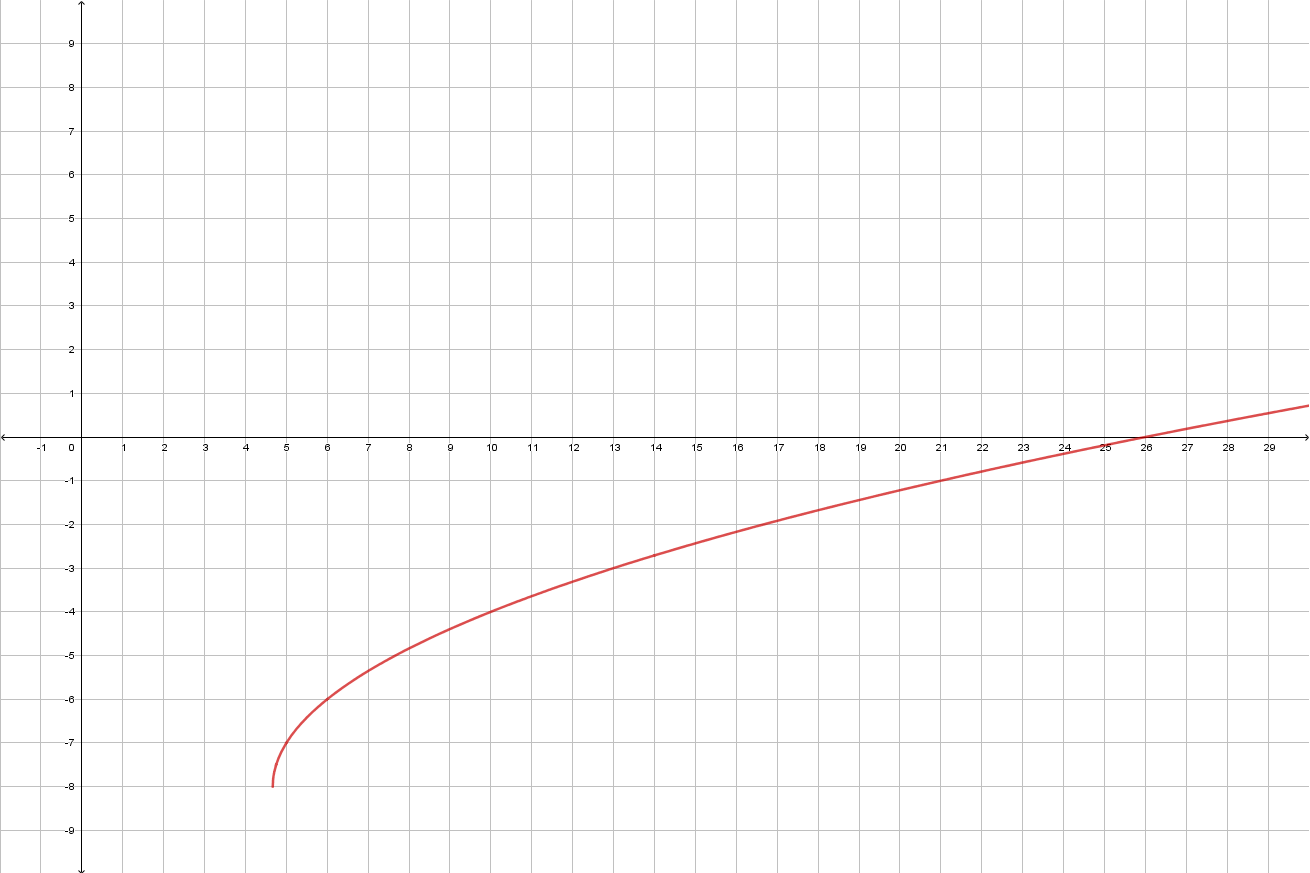
\includegraphics[width=3in]{2330.png}
	
	(a) It appears that the function has a zero at $x = 26$. \\
	(b) \begin{flalign*}
	\sqrt{3x - 14} - 8 &= 0 & \\
	\sqrt{3x - 14} &= 8 & \\
	3x - 14 &= 64 & \\
	3x &= 78 & \\
	x &= 26
	\end{flalign*}
	
	% \vspace{}
	\vfill % \newpage
	
	\begin{bex}{2.3.36}
		{
			
		}
	\end{bex} \vspace{-8pt}
	
	% My answer here
	Increasing: $(-\infty, 0) \cup (2, \infty)$ \\
	Decreasing: $(0, 2)$ \\
	There are no open intervals on which the function is constant.
	
	% \vspace{}
	\vfill % \newpage
	
	\begin{bex}{2.3.40}
		{
			
		}
	\end{bex} \vspace{-8pt}
	
	% My answer here
	Increasing: $(-\infty, 0) \cup (2, \infty)$ \\
	There are no open intervals on which the function is decreasing. \\
	Constant: $(0, 2)$
	
	% \vspace{}
	\vfill % \newpage
	
	\begin{bex}{2.3.52}
		{
			
		}
	\end{bex} \vspace{-8pt}
	
	% My answer here
	Using the Extremum tool in GeoGebra, I found the following relative extrema: \\
	Maximum: $(-0.15, 1.08)$ \\
	Minimum: $(2.15, -5.08)$
	
	% \vspace{}
	\vfill \newpage
	
	\begin{bex}{2.3.72}
		{
			
		}
	\end{bex} \vspace{-32pt}
	
	% My answer here
	\begin{flalign*}
	f(-x) &= (-x)^3 - 5(-x) & \\
	&= -x^3 + 5x & \\
	&= -\fp{x^3 - 5x} & \\
	&= -f(x)
	\end{flalign*}
	Thus, the function is odd; its graph is symmetric about the origin.
	
	% \vspace{}
	\vfill % \newpage
	
	\begin{bex}{2.3.80}
		{
			
		}
	\end{bex} \vspace{-8pt}
	
	% My answer here
	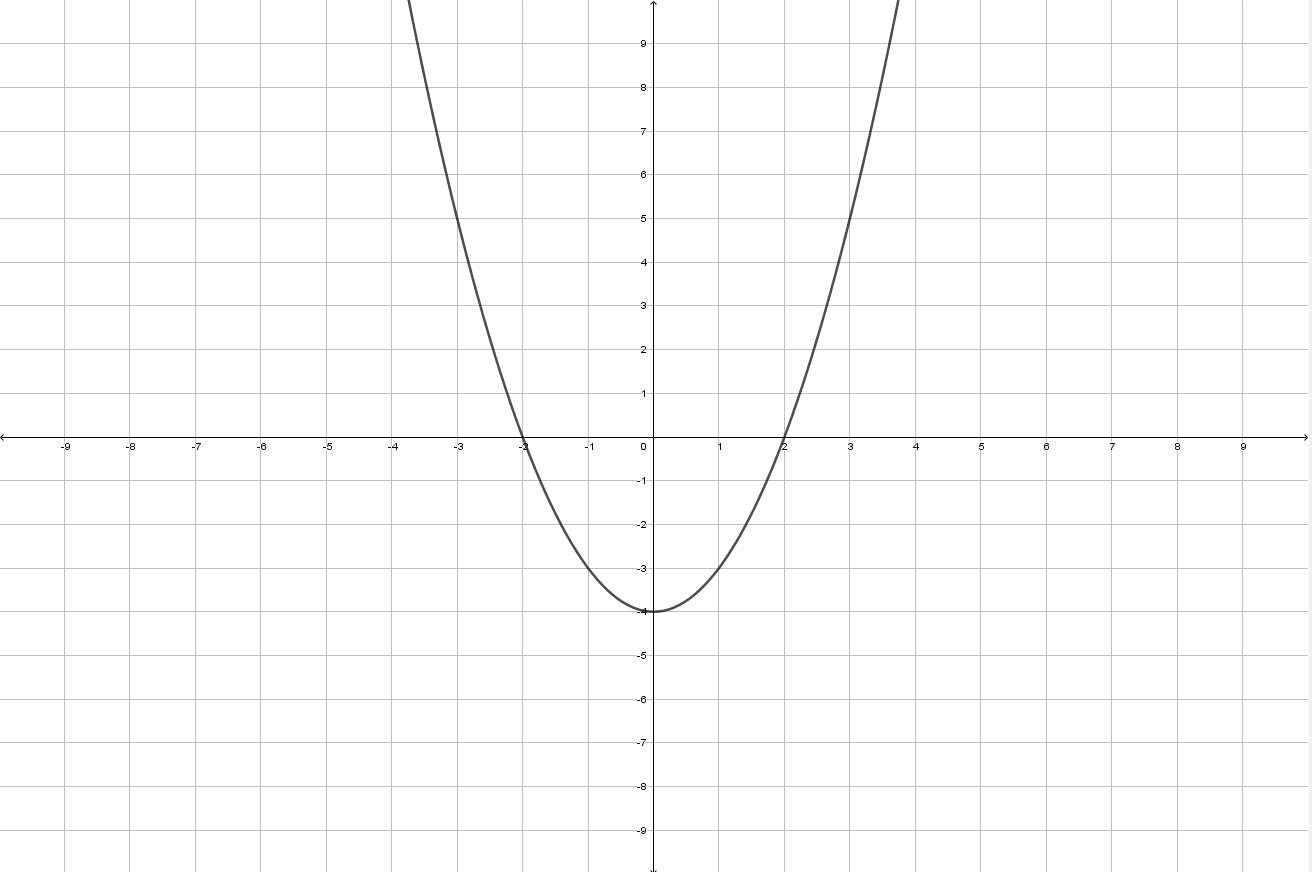
\includegraphics[width=3in]{2380.png}
	
	The graph is symmetric about the $y$-axis, so the function is even. \begin{flalign*}
	f(-x) &= (-x)^2 - 4 & \\
	&= x^2 - 4 & \\
	&= f(x)
	\end{flalign*}
	
	% \vspace{}
	\vfill % \newpage
	
	\begin{bex}{2.4.18}
		{
			
		}
	\end{bex} \vspace{-8pt}
	
	% My answer here
	Using a TI-84 Plus, with default viewing window:
	
	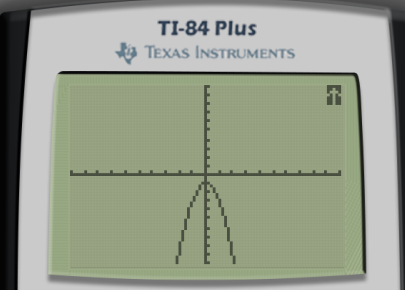
\includegraphics[height=2in]{2418.png}
	
	% \vspace{}
	\vfill \newpage
	
	\begin{bex}{2.4.24}
		{
			
		}
	\end{bex} \vspace{-8pt}
	
	% My answer here
	Using a TI-84 Plus, with default viewing window:
	
	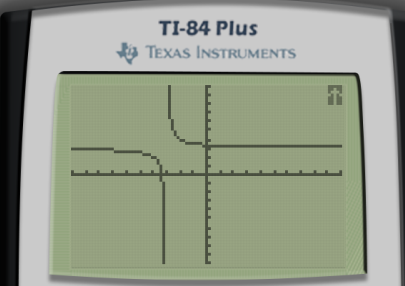
\includegraphics[height=2in]{2424.png}
	
	% \vspace{}
	% \vfill % \newpage
	
	\begin{bex}{2.4.28}
		{
			
		}
	\end{bex} \vspace{-8pt}
	
	% My answer here
	(a) $\step{-2 + 3} = \step{1} = 1$ \\
	(b) $\step{\dfrac12 + 3} = \step{3.5} = 3$ \\
	(c) $\step{4.2 + 3} = \step{7.2} = 7$ \\
	(d) $\step{-21.6 + 3} = \step{-18.6} = -19$
	
	% \vspace{}
	\vfill % \newpage
	
	\begin{bex}{2.4.30}
		{
			
		}
	\end{bex} \vspace{-8pt}
	
	% My answer here
	(a) \vspace{-12pt} \begin{flalign*}
	-7\step{\dfrac18 + 4} + 6 &= -7\step{4.125} + 6 & \\
	&= -7(4) + 6 & \\
	&= -22
	\end{flalign*} (b) \vspace{-12pt} \begin{flalign*}
	-7\step{9 + 4} + 6 &= -7\step{13} + 6 & \\
	&= -7(13) + 6 & \\
	&= -85
	\end{flalign*} (c) \vspace{-12pt} \begin{flalign*}
	-7\step{-4 + 4} + 6 &= -7\step{0} + 6 & \\
	&= -7(0) + 6 & \\
	&= 6
	\end{flalign*} (d) \vspace{-12pt} \begin{flalign*}
	-7\step{\dfrac32 + 4} + 6 &= -7\step{5.5} + 6 & \\
	&= -7(5) + 6 & \\
	&= -29
	\end{flalign*}
	
	% \vspace{}
	\vfill \newpage
	
	\begin{bex}{2.5.10}
		{
			
		}
	\end{bex} \vspace{-8pt}
	
	% My answer here
	Separate file
	
	% \vspace{}
	\vfill % \newpage
	
	\begin{bex}{2.5.12}
		{
			
		}
	\end{bex} \vspace{-8pt}
	
	% My answer here
	(a) The only difference between this graph and the graph of the parent function $f(x) = x^3$ is that this graph has been shifted up one unit. So the equation is $g(x) = x^3 + 1$.
	
	(b) This graph has been shifted one unit down, three units to the right, and reflected across the $y$-axis. So the equation is $g(x) = -\fp{x+3}^3 - 1$
	
	% \vspace{}
	\vfill % \newpage
	
	\begin{bex}{2.5.14}
		{
			
		}
	\end{bex} \vspace{-8pt}
	
	% My answer here
	(a) The graph has been shifted one unit left and seven units down. So the equation is $g(x) = \sqrt{x + 1} - 7$.
	
	(b) The graph has been shifted three units right, four units down. It has also been reflected across both axes. So the equation is $g(x) = -\sqrt{-(x-3)} - 4$. Using the Distributive Property, this simplifies to $g(x) = \sqrt{-x + 3} - 4$.
	
	% \vspace{}
	\vfill % \newpage
	
	\begin{bex}{2.5.16}
		{
			
		}
	\end{bex} \vspace{-8pt}
	
	% My answer here
	The parent function $f(x) = x$ has been vertically constricted by a factor of $2$. The transformed function is $g(x) = \dfrac12 x$.
	
	% \vspace{}
	\vfill % \newpage
	
	\begin{bex}{2.5.18}
		{
			
		}
	\end{bex} \vspace{-8pt}
	
	% My answer here
	The parent function $f(x) = \step{x}$ has been shifted up four units. The transformed function is $g(x) = \step{x} + 4$.
	
	% \vspace{}
	% \vfill % \newpage
	
	\begin{bex}{2.5.20}
		{
			
		}
	\end{bex} \vspace{-8pt}
	
	% My answer here
	The parent function $f(x) = \av{x}$ has been shifted two units to the left. The transformed function is $g(x) = \av{x+2}$.
	
	% \vspace{}
	% \vfill % \newpage
	
	\begin{bex}{2.5.44}
		{
			
		}
	\end{bex} \vspace{-8pt}
	
	% My answer here
	We have that $h = 4$ and $k = -8$. So $f(x) = \av{x - 4} - 8$.
	
	% \vspace{}
	\vfill % \newpage
	
	\begin{bex}{2.5.46}
		{
			
		}
	\end{bex} \vspace{-8pt}
	
	% My answer here
	We have that $k = -9$ and since the graph is reflected across both axes, the function is of the form $g(x) = -f(-x) + k$. The function is $f(x) = -\sqrt{-x} - 9$.
	
	% \vspace{}
	\vfill \newpage
	
	\begin{bex}{2.6.8}
		{
			
		}
	\end{bex} \vspace{-8pt}
	
	% My answer here
	(a) $f + g = 3x + 1 + x^2 - 16 = x^2 + 3x - 15$ \\
	(b) $f - g = 3x + 1 - (x^2 - 16) = -x^2 + 3x + 17$ \\
	(c) \begin{flalign*}
	fg &= (3x + 1)(x^2 - 16) & \\
	&= 3x^3 - 48x + x^2 - 16 & \\
	&= 3x^3 + x^2 - 48x - 16
	\end{flalign*}
	(d) $\dfrac{f}{g} = \dfrac{3x + 1}{x^2 - 16}$; domain is $x \neq \pm 4$.
	
	% \vspace{}
	\vfill % \newpage
	
	\begin{bex}{2.6.12}
		{
			
		}
	\end{bex} \vspace{-8pt}
	
	% My answer here
	(a) \begin{flalign*}
	f + g &= \dfrac{2}{x} + \dfrac{1}{x^2 - 1} & \\
	&= \dfrac{2\fp{x^2 - 1} + x}{x^2 - 1}
	\end{flalign*}
	(b) \begin{flalign*}
	f - g &= \dfrac{2}{x} - \dfrac{1}{x^2 - 1} & \\
	&= \dfrac{2\fp{x^2 - 1} - x}{x^2 - 1}
	\end{flalign*}
	(c) $fg = \dfrac{2}{x(x^2 - 1)}$ \\
	(d) \begin{flalign*}
	\dfrac{f}{g} &= \dfrac{\dfrac{2}{x}}{\dfrac{1}{x^2 - 1}} & \\
	&= \dfrac{2}{x}\cdot \dfrac{x^2 - 1}{1} & \\
	&= \dfrac{2\fp{x^2 - 1}}{x}
	\end{flalign*}
	
	% \vspace{}
	\vfill \newpage
	
	\begin{bex}{2.6.14}
		{
			
		}
	\end{bex} \vspace{-8pt}
	
	% My answer here
	$f + g = x + 3 + \fp{x^2 - 2} = x^2 + x + 1$
	
	So $\fp{f + g}(-1) = (-1)^2 + (-1) + 1 = 1 - 1 + 1 = 1$.
	
	% \vspace{}
	\vfill % \newpage
	
	\begin{bex}{2.6.22}
		{
			
		}
	\end{bex} \vspace{-8pt}
	
	% My answer here
	$\dfrac{f}{g} = \dfrac{x + 3}{x^2 - 2}, x \neq \pm\sqrt{2}$.
	
	So $\fp{\dfrac{f}{g}}(0) = \dfrac{0 + 3}{0^2 - 2} = -\dfrac32$.
	
	% \vspace{}
	\vfill % \newpage
	
	\begin{bex}{2.6.30}
		{
			
		}
	\end{bex} \vspace{-8pt}
	
	% My answer here
	(a) \begin{flalign*}
	f\circ g &= f\fp{g(x)} & \\
	&= f\fp{x + 7} & \\
	&= -4\fp{x + 7} & \\
	&= -4x - 28
	\end{flalign*}
	(b) \begin{flalign*}
	g\circ f &= g\fp{f(x)} & \\
	&= g\fp{-4x} & \\
	&= -4x + 7
	\end{flalign*}
	(c) \begin{flalign*}
	g\circ g &= g\fp{g(x)} & \\
	&= g\fp{x + 7} & \\
	&= \fp{x + 7} + 7 & \\
	&= x + 14
	\end{flalign*}
	% \vspace{}
	\vfill \newpage
	
	\begin{bex}{2.6.32}
		{
			
		}
	\end{bex} \vspace{-8pt}
	
	% My answer here
	(a) \begin{flalign*}
	f\circ g &= f\fp{g(x)} & \\
	&= f\fp{x^4} & \\
	&= 3x^4
	\end{flalign*}
	(b) \begin{flalign*}
	g\circ f &= g\fp{f(x)} & \\
	&= g(3x) & \\
	&= \fp{3x}^4 & \\
	&= 81x^4
	\end{flalign*}
	(c) \begin{flalign*}
	g\circ g &= g\fp{g(x)} & \\
	&= g\fp{x^4} & \\
	&= \fp{x^4}^4 & \\
	&= x^{16}
	\end{flalign*}
	
	% \vspace{}
	\vfill % \newpage
	
	\begin{bex}{2.6.48}
		{
			
		}
	\end{bex} \vspace{-8pt}
	
	% My answer here
	(a) $\fp{f\circ g}(1) = f\fp{g(1)}$. Looking at the graph of $g$, we see that $g(1) = 3$. So the answer is $f(3) = 2$.
	
	(b) $\fp{g\circ f}(3) = g\fp{f(3)}$. Looking at the graph of $f$, we see that $f(3) = 2$. So the answer is $g(2) = 2$.
	
	% \vspace{}
	\vfill % \newpage
	
	\begin{bex}{2.6.58}
		{
			
		}
	\end{bex} \vspace{-8pt}
	
	% My answer here
	(a) The profit of a company is found by subtracting costs from revenue. So \begin{flalign*}
	P &= R - C & \\
	&= 341 + 3.2t - \fp{254 - 9t + 1.1t^2} & \\
	&= -1.1t^2 + 12.2t + 87
	\end{flalign*}
	
	% \vspace{}
	\vfill \newpage
	
	\begin{bex}{2.7.16}
		{
			
		}
	\end{bex} \vspace{-32pt}
	
	% My answer here
	\begin{flalign*}
	f\circ g &= f\fp{g(x)} & \\
	&= f\fp{-\dfrac{2x + 8}{3}} & \\
	&= -\dfrac32\fp{-\dfrac{2x + 8}{3}} - 4 & \\
	&= \dfrac{2(x + 4)}{2} - 4 & \\
	&= x + 4 - 4 & \\
	&= x & \checkmark \\
	g\circ f &= g\fp{f(x)} & \\
	&= g\fp{-\dfrac32 x - 4} & \\
	&= -\dfrac{2\fp{-\dfrac32 x - 4} + 8}{3} & \\
	&= -\dfrac{-3x - 8 + 8}{3} & \\
	&= \dfrac{3x}{3} & \\
	&= x & \checkmark
	\end{flalign*}
	
	% \vspace{}
	\vfill % \newpage
	
	\begin{bex}{2.7.19}
		{
			
		}
	\end{bex} \vspace{-8pt}
	
	% My answer here
	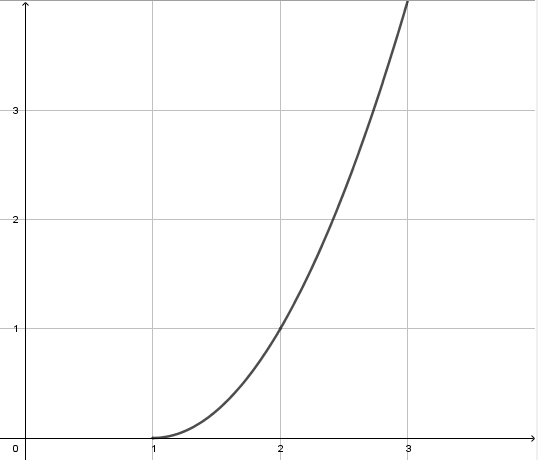
\includegraphics[width=3in]{2719.png}
	
	% \vspace{}
	\vfill \newpage
	
	\begin{bex}{2.7.22}
		{
			
		}
	\end{bex} \vspace{-8pt}
	
	% My answer here
	(a) \begin{flalign*}
	g\circ f &= f(2x) & \\
	&= \dfrac{2x}{2} & \\
	&= x & \checkmark \\
	f\circ g &= g\fp{\dfrac{x}{2}} & \\
	&= 2\fp{\dfrac{x}{2}} & \\
	&= x & \checkmark
	\end{flalign*}
	(b) 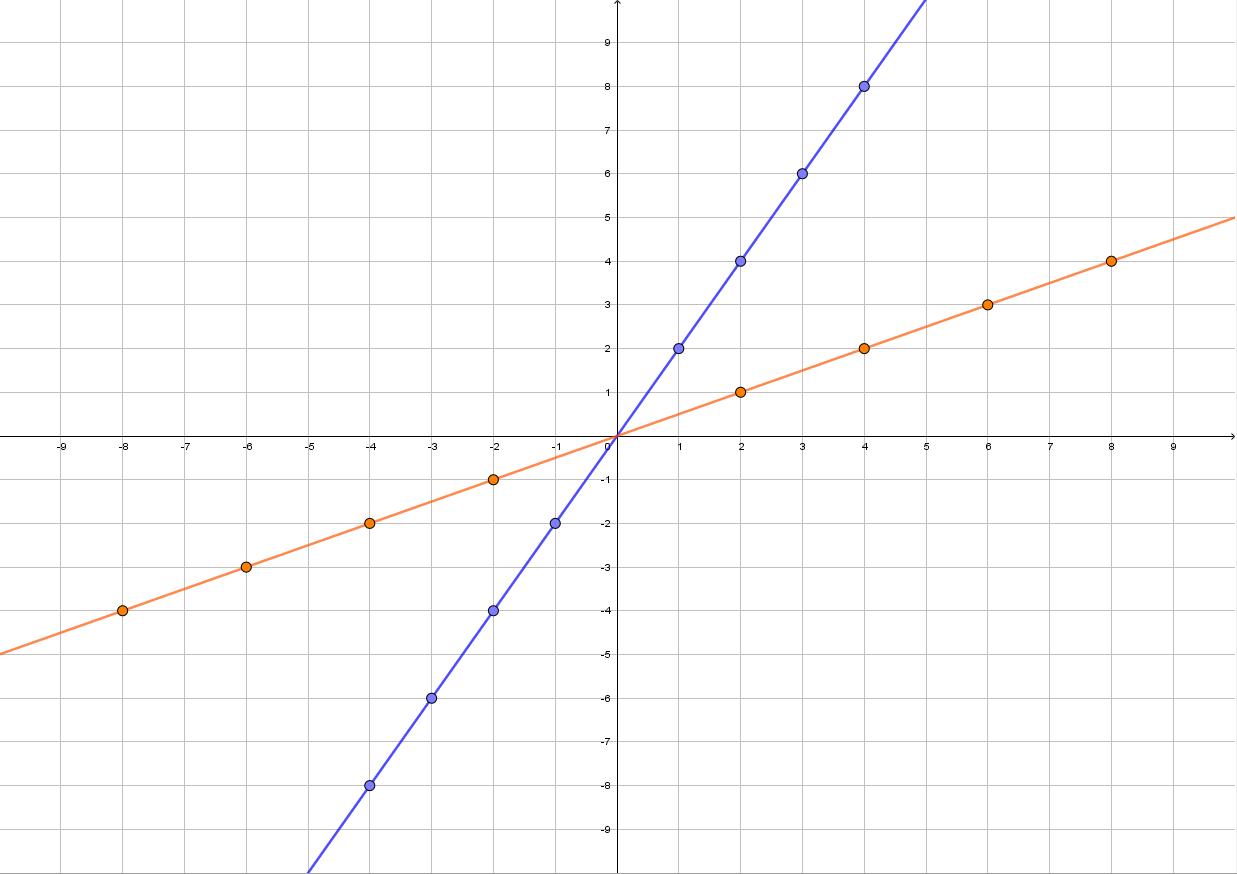
\includegraphics[width=3in]{2722b.png} \\
	We can see that whenever a blue point $(x, y)$ is on the graph of $g(x)$, the point $(y, x)$ is on the graph of $f(x)$.
	
	% \vspace{}
	\vfill \newpage
	
	\begin{bex}{2.7.26}
		{
			
		}
	\end{bex} \vspace{-8pt}
	
	% My answer here
	(a) \begin{flalign*}
	f\circ g &= f\fp{\sqrt[3]{3x}} & \\
	&= \dfrac{\fp{\sqrt[3]{3x}}^3}{3} & \\
	&= \dfrac{3x}{3} & \\
	&= x & \checkmark \\
	g \circ f &= g\fp{\dfrac{x^3}{3}} & \\
	&= \sqrt[3]{3\fp{\dfrac{x^3}{3}}} & \\
	&= \sqrt[3]{x^3} & \\
	&= x & \checkmark
	\end{flalign*}
	(b) 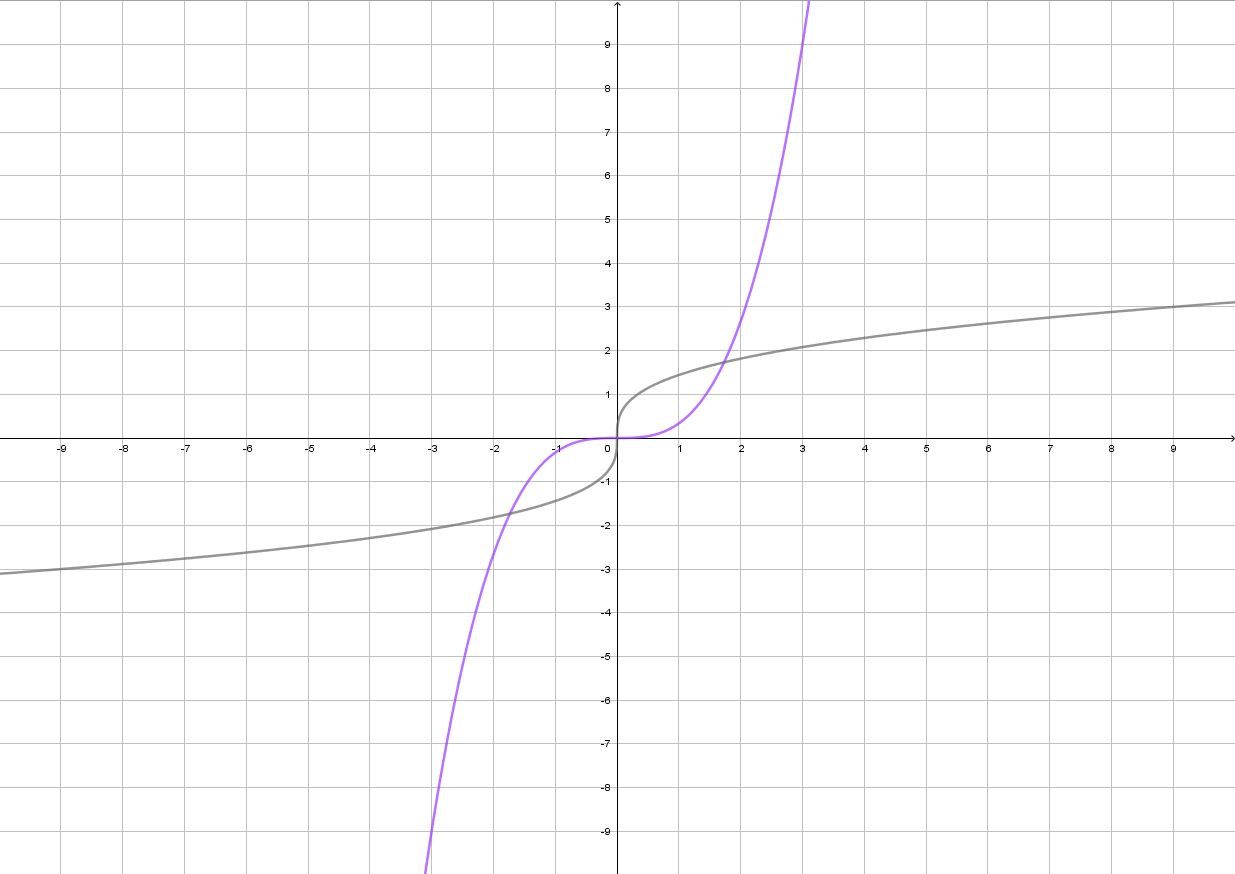
\includegraphics[width=3in]{2726b.png}
	
	% \vspace{}
	\vfill % \newpage
	
	\begin{bex}{2.7.36}
		{
			
		}
	\end{bex} \vspace{-8pt}
	
	% My answer here
	\begin{tabular}{|c|c|c|c|c|c|c|} \hline
		$x$ & 10 & 5 & 0 & -5 & -10 & -15 \\ \hline
		$f^{-1}(x)$ & -3 & -2 & -1 & 0 & 1 & 2 \\ \hline
	\end{tabular}
	
	% \vspace{}
	\vfill % \newpage
	
	\begin{bex}{2.7.42}
		{
			
		}
	\end{bex} \vspace{-8pt}
	
	% My answer here
	The function does have an inverse function, as no horizontal line intersects the graph at more than one location.
	
	% \vspace{}
	\vfill \newpage
	
	\begin{bex}{2.7.44}
		{
			
		}
	\end{bex} \vspace{-8pt}
	
	% My answer here
	The function does not have an inverse since the horizontal line $y  = 4$ intersects the graph at infinitely many locations.
	
	% \vspace{}
	% \vfill % \newpage
	
	\begin{bex}{2.7.56}
		{
			
		}
	\end{bex} \vspace{-8pt}
	
	% My answer here
	The function's graph fails the Horizontal Line Test, so it does not have an inverse.
	
	% \vspace{}
	% \vfill % \newpage
	
	\begin{bex}{2.7.58}
		{
			
		}
	\end{bex} \vspace{-8pt}
	
	% My answer here
	The function's graph passes the Horizontal Line Test, so it does have an inverse. \begin{flalign*}
	y &= 3x + 5 & \\
	x &= 3y + 5 & \\
	3y &= x - 5 & \\
	y &= \dfrac{x - 5}{3} & \\
	f^{-1}(x) &= \dfrac{x - 5}{3}
	\end{flalign*}
	
	% \vspace{}
	% \vfill % \newpage
	
	
	
\end{document}